\documentclass{scrartcl}
\usepackage{physics}   % Matrixes and Dirac-notation
\usepackage{amsmath}   % Binear equations
\usepackage{booktabs}  % Tabs
\usepackage{graphicx}  % Pictures/figures
\usepackage{listings}  % Source code
\usepackage{color}     % Colors
\usepackage{float}

\definecolor{dkgreen}{rgb}{0,0.6,0}
\definecolor{gray}{rgb}{0.5,0.5,0.5}
\definecolor{mauve}{rgb}{0.58,0,0.82}

%Defining source code
\lstset{frame=tb,
  language=Python,
  aboveskip=3mm,
  belowskip=3mm,
  showstringspaces=false,
  columns=flexible,
  basicstyle={\small\ttfamily},
  numbers=none,
  numberstyle=\tiny\color{gray},
  keywordstyle=\color{blue},
  commentstyle=\color{dkgreen},
  stringstyle=\color{mauve},
  breaklines=true,
  breakatwhitespace=true,
  tabsize=3
}
\begin{document}
\begin{titlepage}
	\centering
	{\scshape\LARGE $\star$  \par}
	\vspace{4cm}
	{\scshape\huge FYS2160 - Thermal Physics  \par}
	\vspace{1cm}
	{\scshape\Large Oblig 01\par}
	\vspace{2cm}
	{\Large\itshape Even Marius Nordhagen\par}
	\vfill
	{\large \today\par}
\end{titlepage}
\section{Introduction}
The purpose of this problem set is to learn making simplified models of the Einstein crystal and the spin system. First we are finding the multiplicity of each macrostate, just to find which macrostate that is the most probable, both analytical and numerical. We are also finding expressions for the entropy by using Boltzmann's formula, and from that we can determine the temperature.\par\vspace{3mm}
Sometimes the mathematics is taking the attention from the underlying physics, but that is not good when you are writing a physic rapport. Therefore I will try to keep focus on the formalism and the physic aspects, and just use the mathematics as a tool.\par\vspace{3mm}
All the script are coded in Python, and they can be found in the appendices in the back of this problem set.
\newpage

\section{Part I}
In Part I we take a closer look at the Einstein crystal (also called an ideal crystal) and how energy can move when we have one and two subsystems. We are making some assumptions which simplify the reality a lot, but even though these seems to be rough, they normally fit well with the exact solution.  
\subsection*{a)}
So, we have 3 different oscillators with total energy 3. The possible combinations should be:
\begin{table}[!htbp]
 \centering
 \begin{tabular}{ccc}
   \toprule
   $N_x$ & $N_y$ & $N_z$\\
   \midrule
   3 & 0 & 0\\
   0 & 3 & 0\\
   0 & 0 & 3\\
     &   &  \\
   2 & 1 & 0\\
   2 & 0 & 1\\
   1 & 2 & 0\\
   0 & 2 & 1\\
   1 & 0 & 2\\
   0 & 1 & 2\\
     &   &  \\
   1 & 1 & 1\\
   \bottomrule
 \end{tabular}
 \caption{All microstates for a system with 3 oscillators and 3 units of energy.}
 \label{tab:table1}
\end{table}
\subsection*{b)}
The general formula for the multiplicity of an Einstein solid with $N$ oscillators and total energy $q$ is
\begin{equation}
\Omega(N,q)=\binom{q+N-1}{q}=\frac{(q+N-1)!}{q!(N-1)!}
\end{equation}
By inserting $N=3$ and $q=3$, I should get $\Omega(N,q)=10$ if I did the previous exercise in the right way: 
$$\Omega(3,3)=\frac{5!}{3!2!}=\frac{120}{12}=\underline{10}$$
Oh yeah!
\subsection*{c)}
For a system with two subsystems where subsystem A has $N_A=2$ oscillators and $q_A=5$ energy units, and subsystem B has $N_B=2$ oscillators and $q_B=1$ energy unit, the possible microstates are:
\begin{table}[!htbp]
 \centering
 \begin{tabular}{cccc}
   \toprule
   $N_{A1}$ & $N_{A2}$ & $N_{B1}$ & $N_{B2}$\\
   \midrule
   5 & 0 & 1 & 0\\
   5 & 0 & 0 & 1\\
   0 & 5 & 1 & 0\\
   0 & 5 & 0 & 1\\
     &   &   &  \\
   4 & 1 & 1 & 0\\
   4 & 1 & 0 & 1\\
   1 & 4 & 1 & 0\\
   1 & 4 & 0 & 1\\
     &   &   &  \\
   3 & 2 & 1 & 0\\
   3 & 2 & 0 & 1\\
   2 & 3 & 1 & 0\\
   2 & 3 & 0 & 1\\
   \bottomrule
 \end{tabular}
 \caption{All microstates for a system with two subsystems, where $N_A=2$, $N_B=2$, $q_A=5$ and $q_B=1$.}
 \label{tab:table2}
\end{table}

\subsection*{d)}
The number of possible values for $q_A$ is equal to the number of macrostates, and there can be shown that this number is always $q+1$ for a system of two oscillators (it does not depend on what $N_A$ and $N_B$ are). This means that in our case we have 7 possible values of $q_A$ (and 7 possible values of $q_B$ since $q = q_A + q_B$). The possible values are:
\begin{table}[!htbp]
 \centering
 \begin{tabular}{cc}
   \toprule
   $q_A$ & $q_B$\\
   \midrule
   6 & 0\\
   5 & 1\\
   4 & 2\\
   3 & 3\\
   2 & 4\\
   1 & 5\\
   0 & 6\\
   \bottomrule
 \end{tabular}
 \caption{All possible macrostates for a system of two subsystems where $q=6$.}
 \label{tab:table3}
\end{table}
\newpage

\subsection*{e)}
The task of this exercise is to find all the possible microstates for each of the macrostates.\par\vspace{3mm}
First I will do this analytical, and for that I will use the general formula for the multiplicity of an Einstein solid from Equation (1):
\begin{description}
\item [$\boldsymbol{q_A=6:}$] $\Omega(2,6)\cdot\Omega(2,0)=\frac{7!}{6!}\cdot1!=7$
\item [$\boldsymbol{q_A=5:}$] $\Omega(2,5)\cdot\Omega(2,1)=\frac{6!}{5!}\cdot2!=12$
\item [$\boldsymbol{q_A=4:}$] $\Omega(2,4)\cdot\Omega(2,2)=\frac{5!}{4!}\cdot\frac{3!}{2!}=15$
\item [$\boldsymbol{q_A=3:}$] $\Omega(2,3)\cdot\Omega(2,3)=\frac{4!}{3!}\cdot\frac{4!}{3!}=16$
\item [$\boldsymbol{q_A=2:}$] $\Omega(2,2)\cdot\Omega(2,4)=\frac{3!}{2!}\cdot\frac{5!}{4!}=15$
\item [$\boldsymbol{q_A=1:}$] $\Omega(2,1)\cdot\Omega(2,5)=2!\cdot\frac{6!}{5!}=12$
\item [$\boldsymbol{q_A=0:}$] $\Omega(2,0)\cdot\Omega(2,6)=1!\cdot\frac{7!}{6!}=7$
\end{description}
\par\vspace{3mm}I have also done this numerical, by making a program where I'm plotting a histogram with the number of microstates on the y-axis and the different macrostates on the x-axis. For our specific case the plot is like this (\textit{see Figure 1}). 
\begin{figure}[!htbp]
\centering
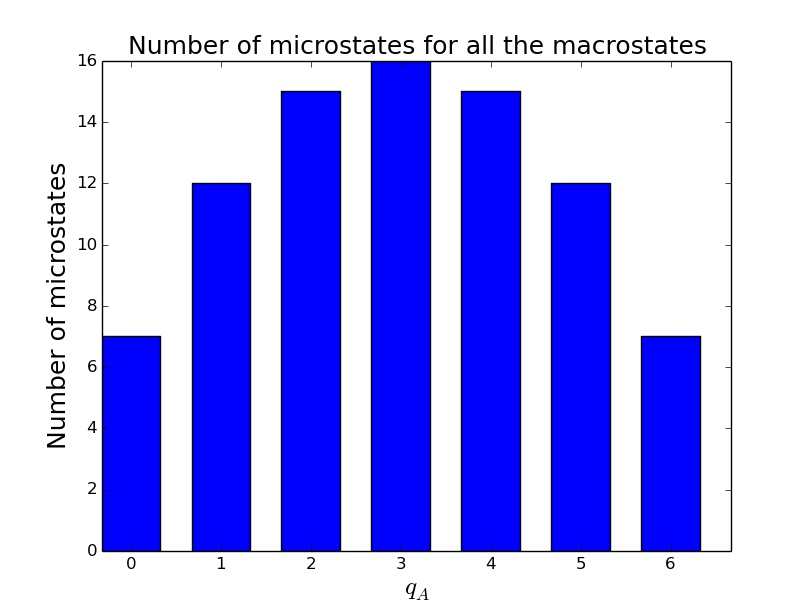
\includegraphics[width=90mm]{oblig1e1.jpg}
\caption{The probability of all the 7 macrostates where we have two subsystems and total energy of 6 units. \label{overflow}}
\end{figure}
\par\vspace{3mm}As we see, my numerical solution is equal to the analytical!\par \vspace{3mm}
The total number of microstates can be found by adding the number of microstates for all the macrostates, or simply by $\Omega(4,6)$. No matter which method we use, we get $84$ possible microstates.\par \vspace{3mm}
By dividing the number of possible microstates for a specific macrostate with the total number of microstates, we get the probability of the macrostate. This can easily be implemented in the program, so one can plot a histogram with the probability columns (\textit{see Figure 2}).
\begin{figure}[!htbp]
\centering
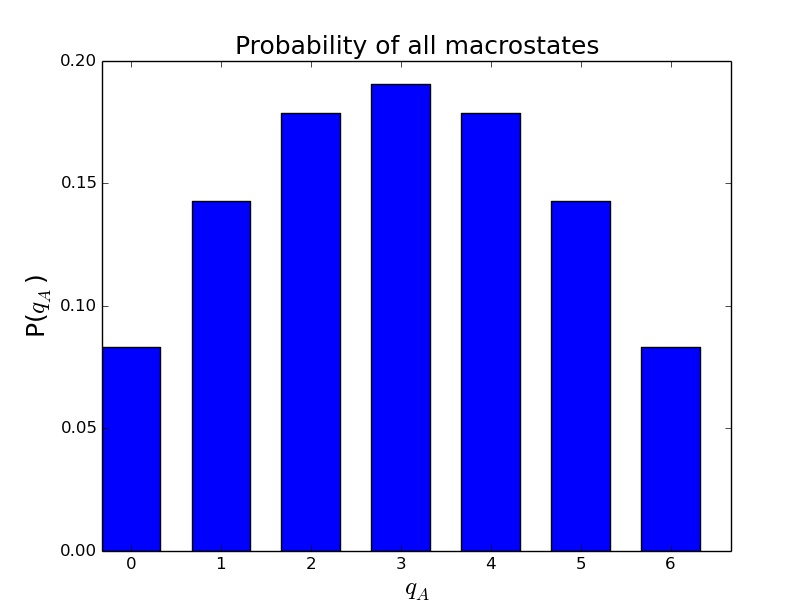
\includegraphics[width=90mm]{oblig1e2.jpg}
\caption{The number of microstates when we have two subsystems and total energy of 6 units. \label{overflow}}
\end{figure}
\par\vspace{3mm}\textit{My program, "oblig1e.py", can be found in Appendix A}

\subsection*{f)}
For the example where $N_A=N_B=2$, $q_A=5$ and $q_B=1$, we saw that the number of microstates is $12$ in the beginning, but it increases to $84$ when the systems are set to thermal contact! The difference is of a factor 7, which is a big difference! This will happened in general, the number of microstates is always greater after thermal contact! Physical the reason is simple: the energy has many more ways to move after thermal contact, and that is what the microstates are intended to show. 
\newpage

\subsection*{g)}
Below you can see the demanded plot (\textit{Figure 3}).
\begin{figure}[!htbp]
\centering
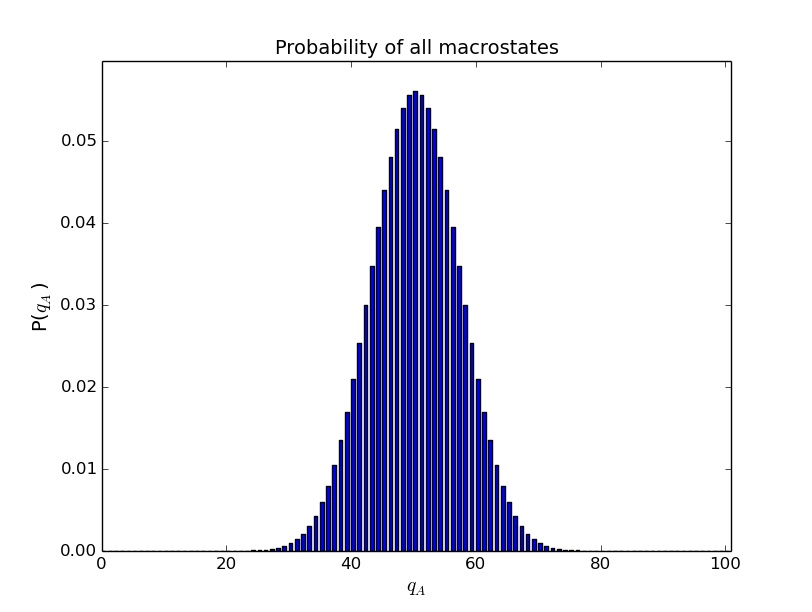
\includegraphics[width=150mm]{oblig1g1.jpg}
\caption{This figure shows the probability on the y-axis (heigth of the columns) and on the x-axis we have 101 columns since we have 101 macrostates \label{overflow}}
\end{figure}
\par\vspace{3mm}
A fundamental law of thermal physics states that the most probable macrostate is when the systems are in equilibrium, and in our case this happens when $q_A=q_B=50$. This is logical since we will have a Gaussian distribution which is max on the half of the interval ($f(x)$ is largest when $x=x_{max}/2$). The exact probability of this state could be found analytical by calculating $\Omega(100,50)/\Omega(100,100)$, but it will obtain a fraction with large factorials, so there is much faster to calculate it numerical. In my Python-script I have printed the probability to the terminal, and I find that it is approach
$$P(q_A=50)\approx \underline{0.056}$$
\textit{I still use the program found in Appendix A, with just changing NA, NB and q.}
\newpage

\subsection*{h)}
In this exercise I am going to show that the natural logarithm of the multiplicity can be simplified to
$$ln\Big(\Omega(N,q)\Big)=N\bigg(ln\frac{q}{N}+1\bigg)$$
If $N\gg 0$, one can make a really good approximation by doing a simplification of Equation (1):
$$\Omega(N,q)=\frac{(q+N-1)!}{(N-1)!}\approx\frac{(q+N)!}{(N)!}$$
since the ratio is almost equal. The next step is to take the natural logarithm of $\Omega(N,q)$:  
$$ln\Omega=ln (q+N)!-ln q!-ln N!$$
Now I have to introduce Stirling's approximation to go future. A much used variant of Stirling's approximation states that
\begin{equation}
ln N!\approx Nln N-N
\end{equation}
By using this on the expression above, I get
$$ln \Omega\approx(q+N)ln (q+N)-(q+N)-qln q+q-Nln N+N=(q+N)ln (q+N)-qln q-Nln N$$
To go even further I have to assume that $q\gg N$. I will try to simplify the first term:
$$ln(q+N)=ln\Bigg[q\bigg(1+\frac{N}{q}\bigg)\Bigg]=ln q+ln\bigg(1+\frac{N}{q}\bigg)\approx ln q+\frac{N}{q}$$
We can make these approximations since the first order Taylor expansion of $ln(1+x)$ gives us 
\begin{equation}
ln(1+x)\approx x
\end{equation}
if $x$ is really small ($|x|\ll 1$). Finally we obtain that
$$ln \Omega \approx N\bigg(ln \frac{q}{N} + 1 + \frac{N}{q}\bigg) \approx \underline{N\bigg(ln \frac{q}{N} + 1\bigg)}$$
we can make the last simplification by assuming that $q\gg N$.

\subsection*{i)}
In general the entropy is given by 
\begin{equation}
S\equiv k ln\omega
\end{equation}
So in our case we have
$$S\approx kN\bigg(ln\Big(\frac{q}{N}\Big)+1\bigg)$$
just by inserting the formula showed in the previous exercise into the definition of entropy.
The reason why we use logarithm, is that $q$ and $N$ often are really large numbers.

\subsection*{j)}
The first thing I want to do is to express $S$ as function of $E$ where $S$ is the entropy and $E$ is the total energy. For that I use the equation from the exercise description which connects $q$ and $E$: 
\begin{equation}
q=\frac{E}{\epsilon}
\end{equation}
Then we obtain:
$$S=Nk\Bigg(ln\bigg(\frac{E}{N\epsilon}\bigg)+1\Bigg)=Nk ln E-Nk ln N\epsilon + Nk$$
The reason I do this is because I already know the temperature formula, and it goes like
\begin{equation}
T\equiv \bigg(\frac{\partial S}{\partial E}\bigg)^{-1}
\end{equation}
The formula is taken from the Lecture Notes\footnote{  "Elementary Thermal Physics using Python", Malthe-Sorenssen, Anders, (2016)} of this course. Since we are deriving with respect to the total energy, we are only interested in terms that include $E$. By inserting the entropy expression, we get
$$T=\bigg(\frac{\partial(NklnE)}{\partial E}\bigg)^{-1}=\bigg(Nk\frac{1}{E}\bigg)^{-1}=\frac{E}{Nk}$$
From this it follows that
$$E=\underline{NkT}$$
This a part of the equipartition theorem, which states that
$$E=\frac{1}{2}kT\cdot n$$
Where n is the number of free degrees (independent subsystems). Because the Einstein crystal has two free degrees for each oscillator, there is easy to see that these expressions are equal.
\newpage

\section{Part II}
In Part II we study how energy is moving in a spin system (in practice an ideal gas). We are first counting the number of microstates, before we use this to find which macrostate that is most probable. The next step is to do some calculations to find three expressions for the multiplicity, and finally we are calculating the entropy and temperature. In conclusion much the same as we did in Part I, but now for an ideal gas.
\subsection*{k)}
Since each of the N spins can have two possible states (+ or -), a N-spin system will have $2^N$ possible microstates. These we can enumerate by + or - for each N, but often we use $\uparrow$ for + and $\downarrow$ for -.

\subsection*{l)}
Net spin is defined by $s=\frac{S_+-S_-}{2}$.\\\\ From the exercise description we have that $E=-S\mu B$, so we can express the total energy as
$$U=-\mu B S_++\mu B S_-=-\mu B(S_+-S_-)=\underline{-2s\mu B}$$
Where I have used the net spin formula. 

\subsection*{m)}
I decided to make a Python script which gives two plots. The first one shows the sum of the microstates. The sum is 0 if the number of spin up particles and equal to the number of spin down, i.e $S_+=S_-=N/2$. It is positive when $S_+ > S_-$ and negative if $S_+ < S_-$. The plot looks like (\textit{See Figure 4}):
\begin{figure}[!htbp]
\centering
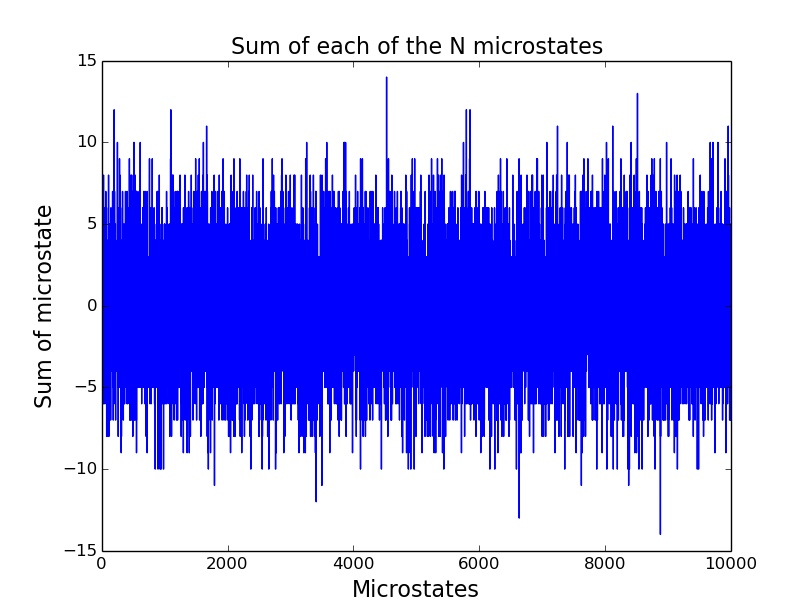
\includegraphics[width=90mm]{oblig1m1.jpg}
\caption{The sum of spin for all the 50 atoms in all the 10000 microstates \label{overflow}}
\end{figure}
\par\vspace{3mm}The remaining plot is the histogram that was demanding in the exercise text (\textit{see Figure 5}).
\begin{figure}[!htbp]
\centering
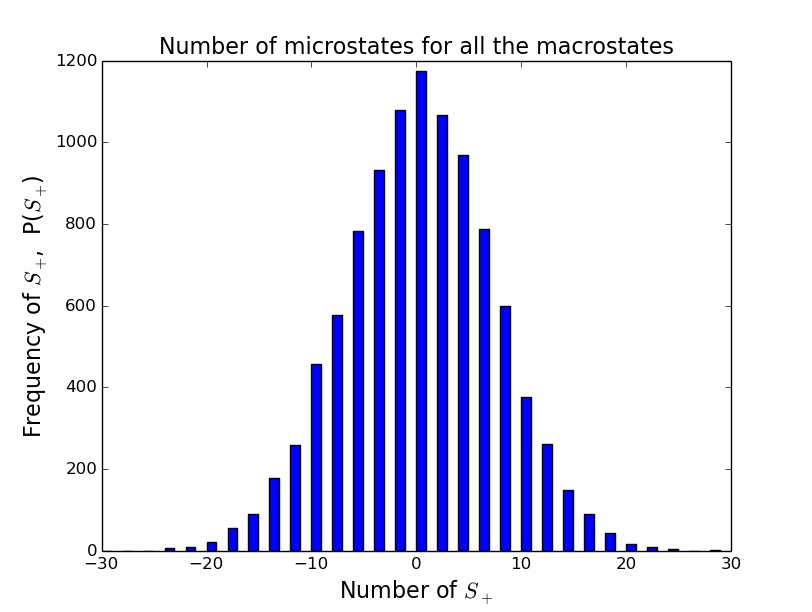
\includegraphics[width=100mm]{oblig1m2.jpg}
\caption{This figure shows the distribution of the sums of all the 10000 microstates\label{overflow}}
\end{figure}
\par\vspace{3mm} As we can see from the Figure, the distribution is approximately gaussian, but with some differences (for example is the middle column a little too high). These differences occurs because we are working with a finite number of random elements, which obviously will give some differences every time they are chosen. The more we increase the number of systems, the better is the gaussian approximation. If we increase the number of systems to infinity, we will have a perfect gaussian distribution. You may wonder why we have that distance between the columns, when the width is set to 0.90 (At least I wondered). The thing is that the energy formula never let us have an odd multiplied with $\mu B$ ($S_+-(N-S_+)$ can never be odd when N is even). Therefore we get quantified values.
 \\\\ \textit{The program, 'oblig1m.py', can be found in Appendix B}
 
\subsection*{n)}
The general formula for number of states is
$$\Omega(N,n)=\binom{N}{n}=\frac{N!}{n!(N-n)!}$$
By inserting into this formula and using that $N=S_++S_-$, we occur
\begin{equation}
\underline{\Omega(N,S_+)=\frac{N!}{S_+!S_-!}}
\end{equation}
Because $N=S_++S_-\Rightarrow S_-=N-S_+$

\subsection*{o)}
We have two connections between $S_+$ and $S_-$, and these are
$$2s=S_+-S_-$$
$$N=S_++S_-$$
By mixing these formulae, one can show that
$$S_+=\frac{N}{2}+s,\quad S_-=\frac{N}{2}-s$$
We can now insert this into Equation (7), and if we do so we get an expression for $\Omega$ which only depends on $N$ and $s$:
\begin{equation}
\underline{\Omega(N,s)=\frac{N!}{(\frac{N}{2}+s)!(\frac{N}{2}-s)!}}
\end{equation}

\subsection*{p)}
One can now start with the expression in the last exercise to show that
$$\Omega(N,s)\approx\Omega(N,0)e^{\frac{-2s^2}{N}}$$
Like the exercise text is hinting to, we have seen something similar in the lectures. On page 81 in the lecture notes, we are starting with a probability distribution on the form
$$P(N,u)=\frac{N!}{(N/2-u)!(N/2+u)!}\cdot2^{-N}$$
Since the probability of a macrostate can be expressed as the multiplicity of the macrostate divided by the total multiplicity, and the total multiplicity is $2^N$ (as we argued for in exercise $k)$), this distribution is equal to the multiplicity formula in exercise $o)$.\par\vspace{3mm}
Equation (4.89) (from the lecture notes) states that 
$$P(N,u)=C(N)exp\bigg(-\frac{u^2}{N/2}\bigg)$$
And because it is just a constant that makes the probability distribution different from the multiplicity, we can also write the formula for multiplicity as
$$\Omega(N,s)=C^*(N)exp\bigg(-\frac{u^2}{N/2}\bigg)$$
where $C^*(N)=C(N)\cdot2^-N$
Actually we do not know anything about the constant $C(N)$, but we can find an expression for $C^*(N)$ by setting $s=0$:
$$C^*(N)=\Omega(N,0)$$
Because $e^0=1$. So then we have shown that 
$$\underline{\Omega(N,s)=\Omega(N,0)exp\bigg(-\frac{2s^2}{N}\bigg)}$$
With some help from the lecture notes.\par\vspace{3mm}
\textit{Comment: We could obtain the same result by solving it analytical, but to get the right factor in the exponent, we need to do Taylor expansion to second order. This is much more work than using the results from the lecture notes.} 
\newpage

\subsection*{q)}
In this exercise I was asked to compare the the multiplicity expression from the previous exercise with the histogram from exercise $m)$. That plot looks like this: 
\begin{figure}[H]
\centering
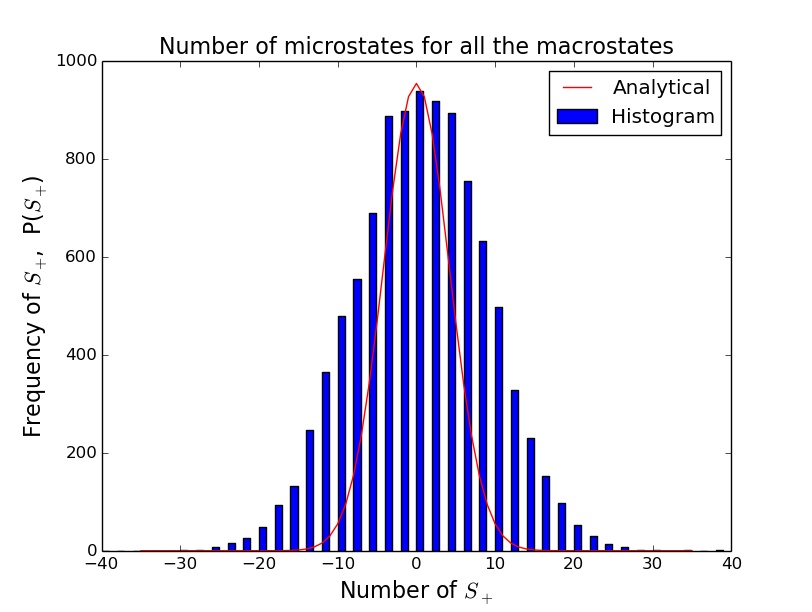
\includegraphics[width=140mm]{oblig1q1.jpg}
\caption{Here I have compared the analytical expression from exercise $p)$ with a histogram of the distribution for the same values of $N$\label{overflow}}\par\vspace{3mm}

My first try was not successful, the analytical solution was way too high! Then I realized that $\Omega(N,0)$ will blow up the function up to the sky, so I decided to normalize the areal to 1. Statistical it will happened because it takes care of all the possible and impossible microstates, but we are just looking for $M$ microstates. \par\vspace{3mm} Then I had to start on new. The idea is that I can calculate the area of the histogram, and multiply the analytical solution with it to get equal area. It makes the plot looking better, but it is still not a perfect plot (the width is too small). I do not know why the error occur.\par\vspace{3mm}
\textit{You can find the program 'oblig1q.py' in Appendix C}
\end{figure}

\subsection*{r)}
In this exercise I will go back to the exact multiplicity formula from \textit{Equation 7}. This is necessary if we want to find exact formulae for entropy and temperature. Since the expression for entropy (\textit{see Equation (4)}) depends on $ln(\Omega)$, an obvious procedure is to start finding an expression for that.
$$ln\Omega(N,S_+)=ln\bigg(\frac{N!}{S_+!(N-S_+)!}\bigg)$$
$$=ln N!-ln S_+! - ln(N-S_+)!$$
$$\approx NlnN-N-S_+ ln S_+ + S_+ - (N-S_+)ln(N-S_+)+N-S_+$$
$$=N\Big(lnN-ln(N-S_+)\Big)-S_+\Big(lnS_+ - ln(N-S_+)\Big)$$
$$=Nln\bigg(\frac{N}{N-S_+}\bigg)-S_+ln\bigg(\frac{S_+}{N-S_+}\bigg)$$
By inserting into the expression for entropy, we occur
$$\underline{S=k\Bigg(Nln\bigg(\frac{N}{N-S_+}\bigg)-S_+ln\bigg(\frac{S_+}{N-S_+}\bigg)\Bigg)}$$

\subsection*{s)}
The last challenge is to find an expression for the temperature. Normally this would correspond to find an expression for $T$, but because the variable $\frac{1}{T}$ is more intuitive, we often find it more interesting. I have already found this formula in \textit{Equation (6)}.
$$\frac{1}{T}=\bigg(\frac{\partial S}{\partial E}\bigg)=\bigg(\frac{\partial S}{\partial S_+}\bigg)\bigg(\frac{\partial S_+}{\partial E}\bigg)$$
Where I also have used the hint from the exercise text. As you can see, I need to express S with respect to $S_+$, and $S_+$ with respect to $E$. The expressions must be
\begin{enumerate}
\item $$S=k\Bigg(Nln\bigg(\frac{N}{N-S_+}\bigg)-S_+ln\bigg(\frac{S_+}{N-S_+}\bigg)\Bigg)$$
\item $$E=-2s\mu B=-(S_+-S_-)\mu B=-S_+\mu B + (N-S_+)\mu B=-2S_+ \mu B +N\mu B$$
\end{enumerate}
So far so good. I will do the calculations in two steps
$$\frac{\partial S}{\partial S_+}=\frac{\partial}{\partial S_+}\left(k\Bigg(Nln\bigg(\frac{N}{N-S_+}\bigg)-S_+ln\bigg(\frac{S_+}{N-S_+}\bigg)\Bigg)\right)$$
To make the derivation correctly we have to be aware. I will split the calculation into two subcalculations just to keep the overview:
$$\frac{\partial}{\partial S_+}\Bigg(kNln\bigg(\frac{N}{N-S_+}\bigg)\Bigg)=kN\bigg(\frac{N-S_+}{N}\bigg)\bigg(\frac{N}{(N-S_+)^2}\bigg)=\frac{kN}{N-S_+}$$
$$\frac{\partial}{\partial S_+}\Bigg(kS_+ln\bigg(\frac{S_+}{N-S_+}\bigg)\Bigg)=kln\bigg(\frac{S_+}{N-S_+}\bigg)+kS_+\bigg(\frac{N-S_+}{S_+}\bigg)\bigg(\frac{N}{(N-S_+)^2}\bigg)$$
$$=kln\bigg(\frac{S_+}{N-S_+}\bigg)+\bigg(\frac{kN}{N-S_+}\bigg)$$
Here I have used the quotient rule to derive the fractions, and in total we get:
$$\frac{\partial S}{\partial S_+}=-kln\bigg(\frac{S_+}{N-S_+}\bigg)=kln\bigg(\frac{N-S_+}{S_+}\bigg)$$
The next step is to derive $S_+$ with respect to $E$, but since I already have an expression for $E$ (with respect to $S_+$), I will take the inverse:
$$\frac{\partial S_+}{\partial E}=\bigg(\frac{\partial E}{\partial S_+}\bigg)^{-1}=\bigg(\frac{\partial}{\partial S_+}\Big(-2S_+ \mu B +N\mu B\Big)\bigg)^{-1}=\bigg(-2\mu B\bigg)^{-1}=-\frac{1}{2\mu B}$$
Finally we obtain the expression for (inverse) temperature:
$$\underline{\frac{1}{T}=\frac{k}{2\mu B}ln\bigg(\frac{N}{S_+}-1\bigg)}$$
\newpage
\section{Appendix A}
Below you can find the code from 'oblig1e.py', that was used in exercise \textit{e)} and \textit{g)}.\par\vspace{3mm} Under the script you can find a description of the code.
\lstinputlisting[language=Python]{oblig1e.py}
Here I will try to explain what I am doing in this program. First I calculate the factorial. I think this little script is simpler than importing factorial from math, but this is individual.\par\vspace{3mm}
The next function is calculating the multiplicity of the Einstein crystal, which I call on in the for loop and storing the multiplicity of every single macrostate into a list. Then I make a histogram with the tools from matplotlib.

%\newpage
\section{Appendix B}
Below you can find the code from 'oblig1m.py', that was used in exercise \textit{m)}.\par\vspace{3mm} Under the script you can find a description of the code.
\lstinputlisting[language=Python]{oblig1m.py}
This program may looks some more ugly than the previous, so I will describe what it is doing. First I create some arrays with different length and shape, just so I can store numbers later. Then I am filling the nested array $F$ with random numbers (either $0$ or $1$, to make the calculations some simpler. For example the sum of an array easily tells me the number of $1's$, or in practice $S_+$). I store the sums into an array $S$, counting the number of each sum in $S$, and storing the numbers of each sum into $P$-array. After that I plot the random numbers and the histogram of the macrostates.  

%\newpage
\section{Appendix C}
Below you can find the program called 'oblig1q.py', which I used in exercise \textit{q)}. The start of the program is similar with the program 'oblig1m.py', which you can find in the previous appendix. Even though I decided to put all the program here since there is some important differences in the main part of the program. \par\vspace{3mm} Under the script you can find a description of the code.
\lstinputlisting[language=Python]{oblig1q.py}
As already said, the start of the program is similar to the previous code, so I will not describe this part (\textit{see Appendix B}). After that I make a function which calculates the multiplicity with $N$ and $s$ as arguments. I decided to remove the constant $2^N$, but this does not matter since I am normalizing later ($2^N$ is a very large number when $N$ is large). Then I have a for-loop that is calling on $Omega(N,s)$, with help from the list $sl$ which stores all possible values of $s$.The loop also stores the different outcomes from $Omega(N,s)$ in an array, which is normalized by dividing on the sum of the array.\par\vspace{3mm}
There can be shown that the total area of the histogram is equal to $M$. This is because each of the columns has width 1 and the total height of the columns is $M$. By multiply the normalized array with $M$, we therefore should get the same area for the histogram and the gaussian, but it does not looks like that. I have to apply that I have no idea what is wrong. \par\vspace{3mm}
The last part consists of different plot commandos.
\end{document}